%----------------------------------------------------------------------------------------
%	PACKAGES AND THEMES
%----------------------------------------------------------------------------------------

\documentclass{beamer}

\mode<presentation> {

    % The Beamer class comes with a number of default slide themes
    % which change the colors and layouts of slides. Below this is a list
    % of all the themes, uncomment each in turn to see what they look like.

    %\usetheme{default}
    %\usetheme{AnnArbor}
    %\usetheme{Antibes}
    %\usetheme{Bergen}
    %\usetheme{Berkeley}
    %\usetheme{Berlin}
    %\usetheme{Boadilla}
    %\usetheme{CambridgeUS}
    %\usetheme{Copenhagen}
    %\usetheme{Darmstadt}
    %\usetheme{Dresden}
    %\usetheme{Frankfurt}
    %\usetheme{Goettingen}
    %\usetheme{Hannover}
    %\usetheme{Ilmenau}
    %\usetheme{JuanLesPins}
    %\usetheme{Luebeck}
    \usetheme{Madrid}
    %\usetheme{Malmoe}
    %\usetheme{Marburg}
    %\usetheme{Montpellier}
    %\usetheme{PaloAlto}
    %\usetheme{Pittsburgh}
    %\usetheme{Rochester}
    %\usetheme{Singapore}
    %\usetheme{Szeged}
    %\usetheme{Warsaw}

    % As well as themes, the Beamer class has a number of color themes
    % for any slide theme. Uncomment each of these in turn to see how it
    % changes the colors of your current slide theme.

    %\usecolortheme{albatross}
    %\usecolortheme{beaver}
    %\usecolortheme{beetle}
    %\usecolortheme{crane}
    %\usecolortheme{dolphin}
    %\usecolortheme{dove}
    %\usecolortheme{fly}
    %\usecolortheme{lily}
    %\usecolortheme{orchid}
    %\usecolortheme{rose}
    %\usecolortheme{seagull}
    %\usecolortheme{seahorse}
    %\usecolortheme{whale}
    %\usecolortheme{wolverine}

    %\setbeamertemplate{footline} % To remove the footer line in all slides uncomment this line
    \setbeamertemplate{footline}[page number] % To replace the footer line in all slides with a simple slide count uncomment this line

    \setbeamertemplate{navigation symbols}{} % To remove the navigation symbols from the bottom of all slides uncomment this line
}

\usepackage{amsmath,amssymb,amsthm,bm}
\usepackage{graphicx}
\usepackage{subcaption}
\usepackage{float}
\usepackage{xifthen}
\usepackage{hyperref}
\hypersetup{
    colorlinks=true,
    linkcolor=blue,
    %filecolor=magenta,
    urlcolor=cyan
}

\newcommand{\der}[3][1]{
	\frac{{\text{d}^{
		\ifthenelse{\equal{#1}{1}}{}{\,#1}
	}
	{#2} }}
	{\text{d} {#3}^{
		\ifthenelse{\equal{#1}{1}}{}{#1}
	}
	}
}

\newcommand{\pder}[3][1]{
	\frac{{\partial^{
		\ifthenelse{\equal{#1}{1}}{}{\,#1}
	}
	{#2}}}
	{\partial {#3}^{
		\ifthenelse{\equal{#1}{1}}{}{#1}
	}
	}
}

\newcommand{\R}{\mathbb{R}}

\renewcommand{\vec}[1]{\bm{#1}}

\newcommand{\norm}[2][2]{\left|\left| #2 \right|\right|_{#1}}


%----------------------------------------------------------------------------------------
%	TITLE PAGE
%----------------------------------------------------------------------------------------

\title[Wave Scattering]{Numerical Simulation of Wave Scattering Off Antennae} % The short title appears at the bottom of every slide, the full title is only on the title page

\author{Jerome Troy} % Your name
\institute[UD] % Your institution as it will appear on the bottom of every slide, may be shorthand to save space
{
University of Delaware\\ % Your institution for the title page
\medskip
}
\date{\today} % Date, can be changed to a custom date

\begin{document}

\begin{frame}
\titlepage % Print the title page as the first slide
\end{frame}

\begin{frame}
\frametitle{Overview} % Table of contents slide, comment this block out to remove it
\tableofcontents % Throughout your presentation, if you choose to use \section{} and \subsection{} commands, these will automatically be printed on this slide as an overview of your presentation
\end{frame}

%----------------------------------------------------------------------------------------
%	PRESENTATION SLIDES
%----------------------------------------------------------------------------------------

%------------------------------------------------

\section{Motivation and Background}
\begin{frame}{The Wave Equation}
    Scalar Waves (eg. sound waves)

$$c^2 \nabla^2 \psi = \pder[2]{\psi}{t}$$

\begin{itemize}
    \item $\psi(\vec{x},t)$ - the amplitude of the wave
    \item $\vec{x} \in \R^2$ - position
    \item $t > 0$ - time
    \item $c$ - the speed of wave propagation
\end{itemize}

Letting $t \mapsto \frac{1}{c} t$ effectively sets $c = 1$
\end{frame}


\begin{frame}{The Antenna Problem}
    Waves emminate from a source

These waves reflect off the antenna in such a way to be directed towards a target

The problem is how to calculate the scattering pattern off an antenna

Setting reflection at the antenna surface ($S_A$)

$$\left.\psi \right|_{S_A} = 0$$

\begin{center}
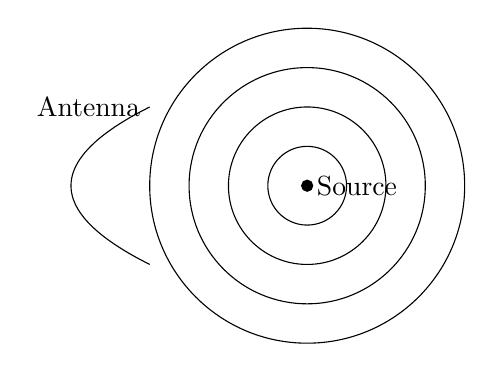
\begin{tikzpicture}
    \filldraw [black] (3,0) circle (2pt) node [anchor=west] {Source};
    \draw [smooth,domain=-1:1,variable=\y] plot({\y*\y},{\y})
    node [anchor=east] {Antenna};
    \draw (3.5,0) arc (0:360:0.5);
    \draw (4,0) arc (0:360:1);
    \draw (4.5,0) arc (0:360:1.5);
    \draw (5,0) arc (0:360:2);
\end{tikzpicture}
\end{center}
\end{frame}

\section{Numerical Methods}

\begin{frame}{Discretization}
    Problem: we cannot simulate an infinite domain!

Will let domain be large enough to minimize reflections off boundaries

$x \in \left[-X,X\right], \quad y \in \left[-Y,Y\right]$

Number of nodes: $M_x, M_y$ in $x$ and $y$ directions respectively

$x_i = -X + ih_x, \quad h_x = \frac{2X}{M_x}, \quad i = 0, 1, ..., M_x$, 
and $y_j = -Y + jh_y, \quad h_y = \frac{2Y}{M_y}, \quad j = 0, 1, ..., M_y$

$$\R^{M_x+1\times M_y+1} \ni \Psi_{ij}(t) \approx \psi(x_i, y_j, t) \implies \der[2]{}{t} \Psi = \nabla^2 \Psi$$

Differentiation Matrices!

$$\nabla^2 \Psi = \left(\pder[2]{}{x} + \pder[2]{}{y}\right) \Psi \mapsto D_{xx} \Psi + \Psi D^T_{yy}$$

Solving 

$$\der[2]{}{t} \Psi = D_{xx} \Psi + \Psi D^T_{yy}, \quad \left.\Psi\right|_{S_A} = 0$$
\end{frame}

%\begin{frame}{Building Differentiation Matrices}
%    Want to build matrix $D_{xx}$ such that $D_{xx} \Psi(t) = \pder[2]{}{x} \psi (\vec{x},t) + O(h^2)$

Interior points:

$$af(x - h) + b f(x) + cf(x + h) = f''(x) + O(h^2)$$

$$\implies a = \frac{2}{h^2}, \quad b = \frac{-4}{h^2}, \quad c = \frac{2}{h^2}$$

End points:

$$a f(x) + bf(x + h) + cf(x + 2h) + df(x + 3h) = f''(x) + O(h^2)$$

$$\implies a = \frac{2}{h^2}, \quad b = -\frac{5}{h^2}, \quad c = \frac{4}{h^2}, \quad d = -\frac{1}{h^2}$$
%\end{frame}

\begin{frame}{Building Differentiation Matrices (continued)}
    Put this all together:

$$D_{xx} = \frac{2}{h^2}\begin{bmatrix}
1 & -\frac{5}{2} & 2 & -\frac{1}{2} \\
1 & -2 & 1 \\
& 1 & -2 & 1 \\
& & \ddots & \ddots & \ddots \\
& & & 1 & -2 & 1 \\
& & \frac{1}{2} & -2 & \frac{5}{2} & -1
\end{bmatrix}$$

For $D_{yy}$ we wish to operate on the rows, so we need to use the transpose!
\end{frame}

\begin{frame}{Verlet Integration}
    How do we solve 

$$\der[2]{}{t} u = f(t,u), \quad u(0) = u_0, \quad u'(0) = v_0, \quad t \geq 0$$

St\"ormer Verlet Integration:

$t_k = k\tau$, $\tau$ time step size, then let $u_k \approx u(t_k)$

Define:

$$u_1 = u_0 + \tau v_0 + \frac{\tau^2}{2} f(t_0,u_0)$$

Then iterate via:

$$u_{k+1} = 2u_{k} - u_{k-1} + \tau^2 f(t_k,u_k), \quad k \geq 1$$

Verlet's method is $O(\tau^2)$ \textbf{citation needed}
\end{frame}

\section{Results}

\begin{frame}{Test Case - No Reflector}
    
\animategraphics[loop,controls,width=\textwidth]{10}
{figures/no-reflector/no-reflector-}{0}{219}

\end{frame}

\begin{frame}{Elliptical Reflector Dish}
    
\animategraphics[loop,controls,width=\textwidth]{10}
{figures/elliptic/elliptic-dish-}{0}{219}

\end{frame}

\begin{frame}{Parabolic Reflector}
    
\animategraphics[loop,controls,width=\textwidth]{10}
{figures/parabolic/parabolic-dish-}{0}{219}

\end{frame}

\begin{frame}{Comparison of Efficiencies}
    \begin{figure}
  \centering
  \begin{subfigure}[b]{0.47\textwidth}
    \includegraphics[width=\textwidth]{figures/elliptic-total-abs-cropped}
    \caption{Elliptic reflector}
    \label{fig:elliptic-distribution}
  \end{subfigure}
  \begin{subfigure}[b]{0.47\textwidth}
    \includegraphics[width=\textwidth]{figures/parabolic-total-abs-cropped}
    \caption{Parabolic reflector}
    \label{fig:parabolic-distribution}
  \end{subfigure}

\end{figure}

\end{frame}

\section{Conclusions}


\begin{frame}{Conclusions}
  \begin{itemize}
  \item St\"ormer Verlet Integration has good accuracy for 2D wave equation
  \item This allows us to solve the equation without factorizing $\nabla^2$ as
  in the Maxwell Equations \cite{fnc-driscoll}
  \item Verified parabolic columnation of energy from focus
\end{itemize}

\end{frame}

\begin{frame}{Thank You!}
    Questions?
\end{frame}

\begin{frame}{References}
  \bibliography{biblio}
  \bibliographystyle{ieeetr}
\end{frame}
\end{document}
